\subsection{Laufrichtungen kombinieren}
Die Charaktersteuerung erfordert je nach Tastatureingabe eine unterschiedliche Bewegungsrichtung. Um dies zu erreichen, wird die Funktion zum Wechseln des verwendeten Modells im Unity ML-Agents Agent genutzt. Mit dieser Funktion wird in der folgenden Implementierung zwischen den separaten Bewegungsmodellen gewechselt, um alle Bewegungsrichtungen mit einer Steuerung abzudecken. Es wird erwartet, dass die Bewegung in die einzelnen Richtungen funktioniert, dass der Läufer jedoch beim Wechsel zwischen den Modellen das Gleichgewicht nicht halten kann. Das Balance Problem bei Übergängen zwischen den Modellen ist darauf zurückzuführen, dass die Bewegungsmodelle separat voneinander trainiert wurden, und der Agent somit im Training den Zustandswechsel bzw. die Zustände der anderen Bewegungsabläufe nie gelernt hat. Der Läufer kann daher durch die plötzliche Veränderung in den Bewegungsabläufen das Gleichgewicht verlieren.

\begin{lstlisting}[caption={Laufrichtung Modell wechseln},captionpos=b,label={lst:laufrichtung_modell_wechsel}]
public override void FixedUpdate() {
    ...    
    agent.targetWalkingSpeed = 5f;
    if (inputVert != 0) //Tastatur Input Vor oder Zurück
    {
        // Vorwärts
        if (inputVert > 0)
        {
            agent.SetModel("Walker", modelForward);
        }
        else // Zurück
        {
            agent.SetModel("Walker", modelBackward);
        }
    }
    else if (inputHor != 0) // Links oder Rechts
    {
        if (inputHor > 0) // Rechts
        {
            agent.SetModel("Walker", modelRight);
        }
        else // Links
        {
            agent.SetModel("Walker", modelLeft);
        }
    }
    else //kein Input -> Auf der Stelle stehen
    {
        agent.targetWalkingSpeed = 0f;
        agent.SetModel("Walker", modelStanding);
    }
    ...
}
\end{lstlisting}

Wie angenommen funktioniert das Bewegen in eine konstante Richtung gut. Beim Wechsel zu einem anderen Modell fällt der Läufer jedoch ohne Ausnahme. Um dieses Problem zu lösen, ergeben sich zwei grundlegende Verfahren. Zum Einen kann versucht werden, die Übergänge zwischen den Modellen zu optimieren. Ein zweiter Ansatz ist, die unterschiedlichen Bewegungsabläufe in einem einzigen Modell anzutrainieren. Im Folgenden wird eine Lösung basierend auf dem zweiten Ansatz entwickelt und ausgewertet.

Der erste Versuch, alle Bewegungsrichtungen in einem Modell anzulernen, wurde von den Methoden der Walker Demo inspiriert. Ähnlich wie beim Laufziel wurde ein zusätzliches Zielobjekt hinzugefügt, das zufällig platziert wurde. Um die Komplexität des Lernprozesses nicht von Anfang an zu hoch anzusetzen, wurde das Blickziel – also die Winkelabweichung zwischen Zielrichtung und Blickrichtung – schrittweise über einen Lehrplan angepasst. Zu Beginn wurde das Blickziel mit einer Winkelabweichung im Bereich von -5 bis 5 Grad platziert, um sicherzustellen, dass der Läufer zunächst nur geringe Anpassungen in der Blickrichtung vornehmen muss. Im Laufe des Trainings wurde dieser Bereich allmählich auf -90 bis 90 Grad erweitert, um die Lernanforderungen schrittweise zu steigern (siehe Codeausschnitt \ref{lst:lehrplan_blickziel}). Das Blickziel wurde jedes Mal neu gesetzt, sobald ein Ziel erreicht wurde.

Diese Methode wurde gewählt, um mit geringer Anfangsschwierigkeit das Erlernen des grundlegenden Verhaltens zu erleichtern. Bei zu großer Anfangsschwierigkeit kann es dazu kommen, dass der Läufer ein falsches Verhalten lernt oder gar keine zielführende Lösung findet. Ein potenzielles Risiko bei diesem Ansatz besteht jedoch darin, dass in der Startphase ein Verhalten gefestigt wird, das in späteren Etappen nicht in der Lage ist, auf größere Abweichungen des Blickwinkels zu adaptieren. Der Erfolg dieses Ansatzes wird davon abhängen, ob der Läufer in der Lage ist, das während der frühen Lernphasen erlernte Verhalten flexibel anzupassen, wenn die Anforderungen in späteren Phasen erhöht werden.

\begin{lstlisting}[caption={ Lehrplan für das Blickziel},captionpos=b,label={lst:lehrplan_blickziel}]
lookAngleLimit:
    curriculum:
      - name: min max 5 degree look target deviation
        completion_criteria:
          measure: progress
          behavior: Walker
          threshold: 0.4
          signal_smoothing: true
        value: 5.0
      - name: min max 30 degree look target deviation
        completion_criteria:
          measure: progress
          behavior: Walker
          threshold: 0.6
          signal_smoothing: true
          require_reset: true
        value: 30.0
      - name: min max 60 degree look target deviation
        completion_criteria:
          measure: progress
          behavior: Walker
          threshold: 0.8
          signal_smoothing: true
          require_reset: true
        value: 60.0
      - name: min max 90 degree look target deviation
        completion_criteria:
          measure: progress
          behavior: Walker
          threshold: 1.0
          signal_smoothing: true
          require_reset: true
        value: 90.0
\end{lstlisting}

Der Läufer lernt einen stabilen Gang (siehe Abbildungen \ref{fig:103_move_target_dir} und \ref{fig:103_reach_target}). Die Winkelabweichung von 5 Grad ist jedoch mit der aktuellen Belohnungsfunktion nahezu zu vernachlässigen. Bereits vor den folgenden Lehreinheiten hat sich ein Verhalten so stark gefestigt, dass die Lehreinheiten keine Wirkung mehr zeigen (siehe Abbildungen \ref{fig:103_look_angle_limit} und \ref{fig:103_look_reward}). Diese Ergebnisse zeigen, dass die Auswirkung der 5 Grad Winkelabweichung zu gering war, um das Verhalten auf Abweichungen der Zielblickrichtung vorzubereiten. Ein weiteres Problem war, dass die initiale Lernepisode zu lang war, wodurch das Verhalten bereits zu stark auf die spezifischen Gegebenheiten der ersten Lernphase angepasst war.

\begin{figure}[H]
  \centering  
    \begin{subfigure}{.49\textwidth}
      \centering  
      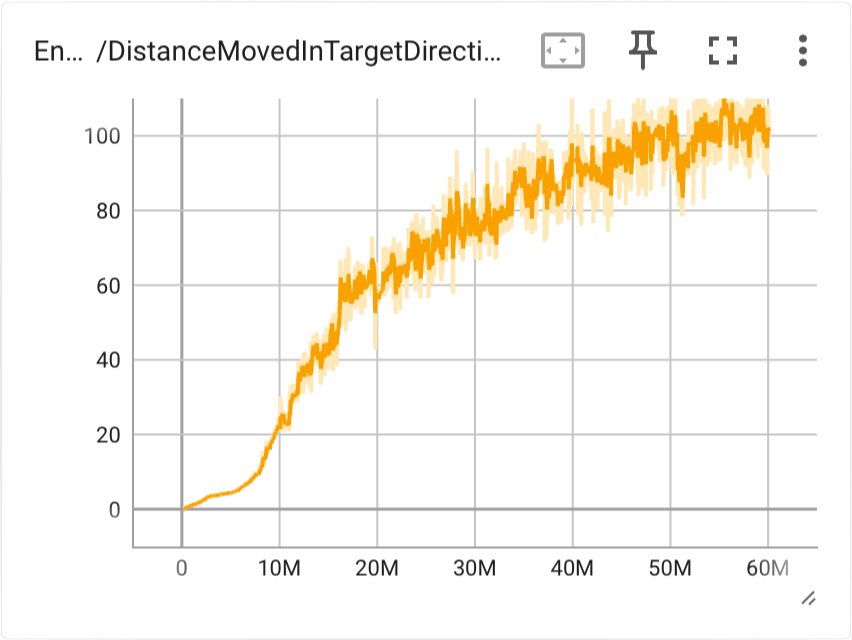
\includegraphics[width=\textwidth]{img/103_move_target_dir}
      \caption{Zurückgelegte Strecke in Zielrichtung}
      \label{fig:103_move_target_dir}
    \end{subfigure}
    \begin{subfigure}{.49\textwidth}
      \centering  
      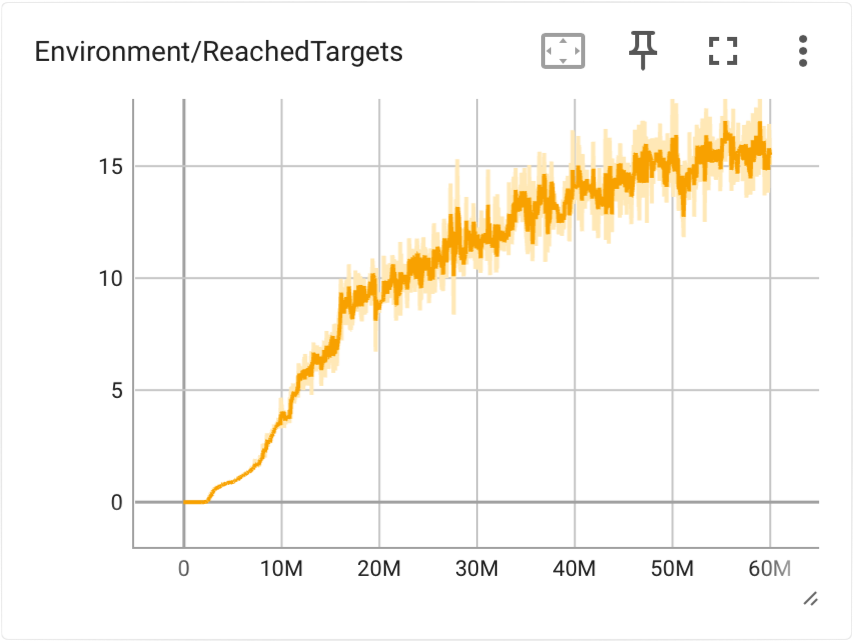
\includegraphics[width=\textwidth]{img/103_reach_target}
      \caption{Erreichte Anzahl an Zielen}
      \label{fig:103_reach_target}
    \end{subfigure}
    \begin{subfigure}{.49\textwidth}
      \centering  
      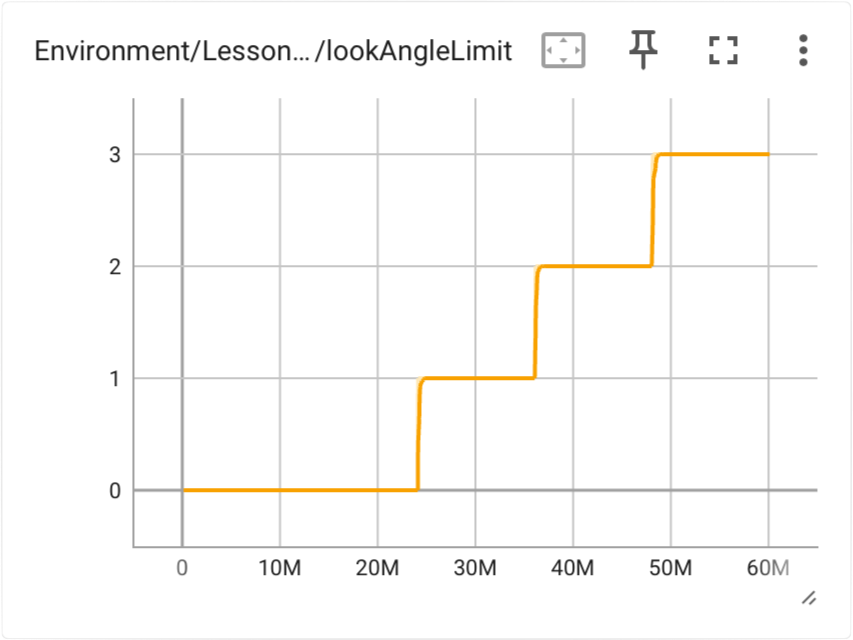
\includegraphics[width=\textwidth]{img/103_look_angle_limit}
      \caption{Aktive Lehreinheit}
      \label{fig:103_look_angle_limit}
    \end{subfigure}
     \begin{subfigure}{.49\textwidth}
      \centering  
      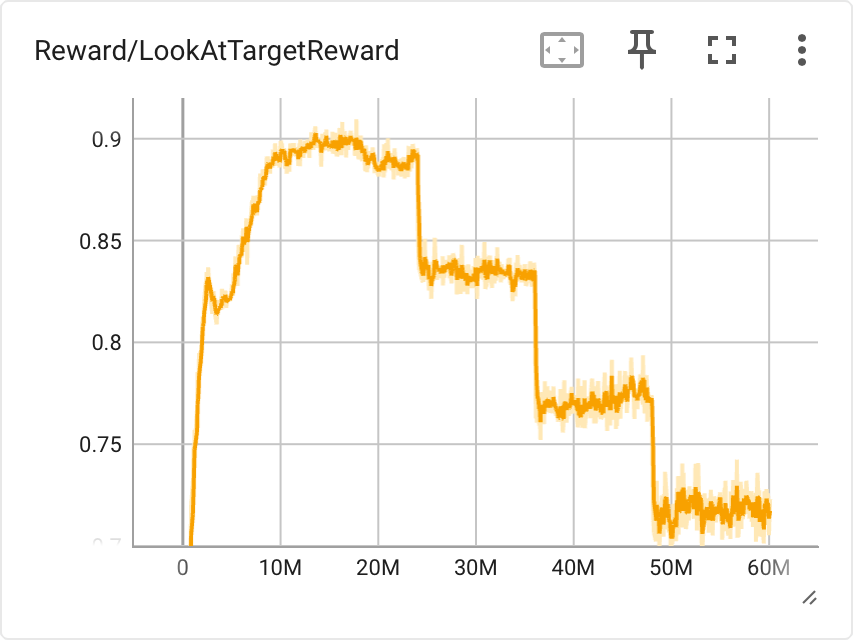
\includegraphics[width=\textwidth]{img/103_look_reward}
      \caption{Blickbelohnung}
      \label{fig:103_look_reward}
    \end{subfigure}
  \caption{Training Blickrichtungsziel mit Lehrplan}
  \label{fig:training_blickrichtungsziel_lehrplan}
\end{figure}

Um von Beginn an ein generell gültiges Verhalten anzutrainieren und somit das Problem der Spezialisierung des Modells auf eine bestimmte Blickrichtung zu umgehen, wurden Trainings ohne Lehrplan durchgeführt. Dabei wurde ein Training mit einer Winkelabweichung von +-90 Grad und eines mit +-180 Grad durchgeführt. In beiden Trainings lernte der Läufer jedoch kaum, seine Blickrichtung an die neue Zielrichtung anzupassen. Insbesondere beim Training mit Winkelabweichungen von bis zu ±180 Grad entdeckte der Läufer eine Möglichkeit, negative Belohnungen zu umgehen, indem er seine Blickrichtung vertikal nach unten ausrichtete. Dies ist möglich, weil die Blickrichtung vertikal nach unten entlang der Y-Achse verläuft. Bei der Berechnung der Blickbelohnung wird die Y-Komponente der Blickrichtung auf 0 gesetzt, da die Zielrichtung ohne Höhenkomponente festgelegt wird, um Höhenunterschiede zwischen Hüfte und Ziel zu ignorieren. Durch dieses Schlupfloch kann der Läufer negative Belohnungen verhindern, ohne seine Gangart nennenswert anzupassen. Diese Beobachtung zeigt eine Schwäche in der aktuellen Belohnungsfunktion, gleichermaßen demonstriert es aber auch gut, wie der Agent lernt. Der Agent hat keinerlei Verständnis über die gelernten Bewegungsabläufe; er versucht lediglich, die Belohnung zu maximieren und nutzt dabei jedes verfügbare Mittel. Im Training findet der Agent so häufig Wege, die bei der Entwicklung vermeintlich sorgfältig gesetzten Ziele zu umgehen. Um dieses Problem zu adressieren, kann die Belohnungsfunktion angepasst oder zusätzliche Belohnungsfunktionen hinzugefügt werden.

\begin{figure}[H]
  \centering  
    \begin{subfigure}{.49\textwidth}
      \centering  
      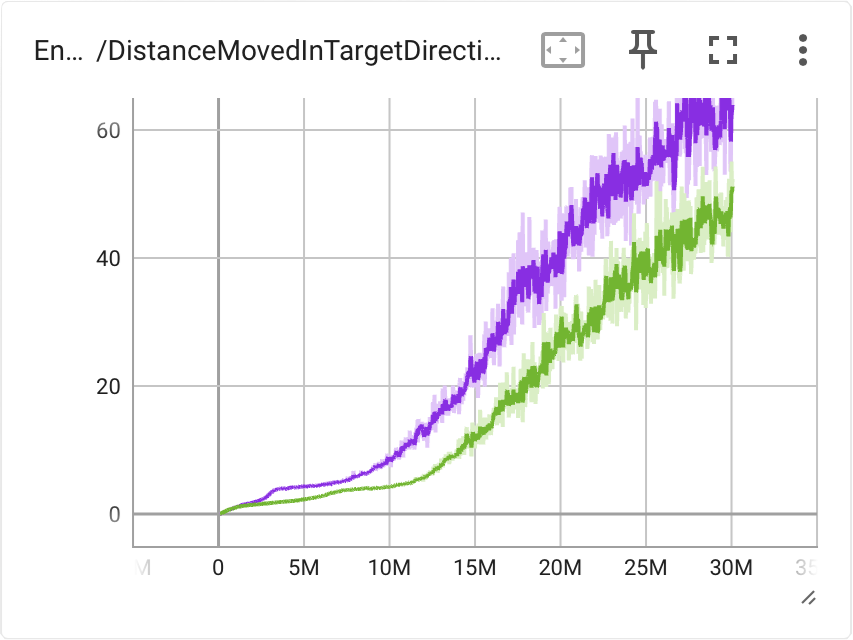
\includegraphics[width=\textwidth]{img/104_105_move_target_dir}
      \caption{Zurückgelegte Strecke in Zielrichtung}
      \label{fig:104_105_move_target_dir}
    \end{subfigure}
    \begin{subfigure}{.49\textwidth}
      \centering  
      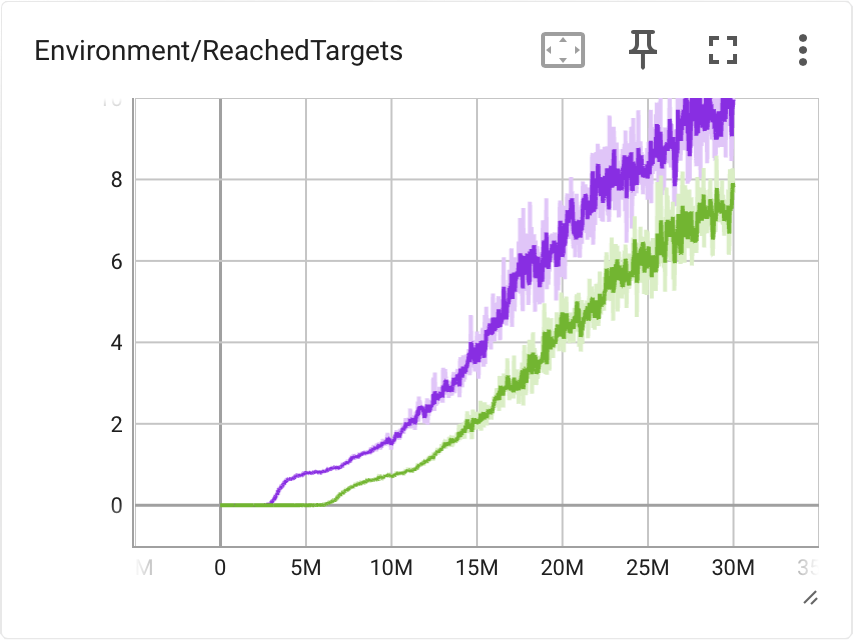
\includegraphics[width=\textwidth]{img/104_105_reach_target}
      \caption{Erreichte Anzahl an Zielen}
      \label{fig:104_105_reach_target}
    \end{subfigure}
    \begin{subfigure}{.49\textwidth}
      \centering  
      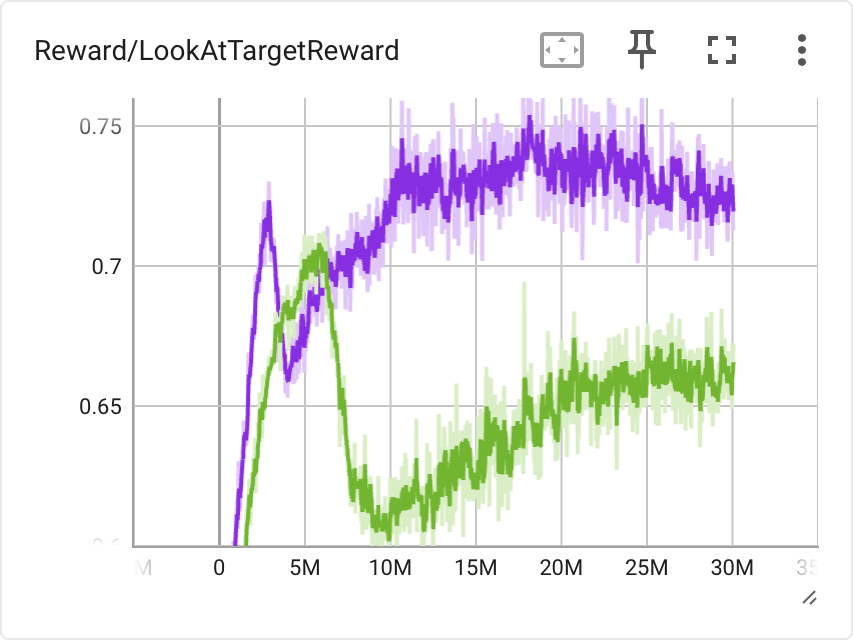
\includegraphics[width=\textwidth]{img/104_105_look_reward}
      \caption{Blickbelohnung}
      \label{fig:104_105_look_reward}
    \end{subfigure}
  \caption{Training Blickrichtungsziel (blau = Winkelabweichung +-90 Grad, grün = Winkelabweichung +-180 Grad)}
  \label{fig:training_blickrichtungsziel}
\end{figure}

Um das Schlupfloch in der Blickbelohnung zu schließen, wurde eine neue Bestrafung eingeführt: die Kopfneigungsbestrafung. Diese Bestrafung sorgt dafür, dass der Läufer für das Neigen des Kopfes bestraft wird, wodurch er gezwungen wird, den Kopf aufrecht zu halten. Im Training mit der neuen Kopfneigungsbestrafung lernt der Läufer jedoch langsamer und findet stattdessen einen neuen Ausweg, um die Belohnungen generell zu optimieren, ohne unterschiedliche Gangarten zu erlernen. Durch die Eigenschaft des Trainings, dass der Winkel zwischen Läufer, Ziel und Blickziel nur bei der Platzierung des Blickziels eingehalten wird, vergrößern sich die Winkel, wenn sich der Läufer dem Ziel nähert, ausnahmslos. Dies führt dazu, dass die beste Lösung für den Läufer darin besteht, sich rückwärts zu bewegen, da die Wahrscheinlichkeit, dass die Winkelabweichung kleiner ist, wesentlich höher ist. Die Abbildung \ref{fig:blickwinkel_änderung} zeigt, wie sich der Blickwinkel ändert, wenn der Läufer sich dem Ziel nähert, und verdeutlicht, warum das rückwärtsgerichtete Gehen eine vorteilhafte Strategie für den Läufer darstellt.

\begin{figure}[H]
  \centering  
    \begin{subfigure}{.3\textwidth}
      \centering  
      \includegraphics[width=\textwidth]{img/blickwinkel_änderung1}
    \end{subfigure}
    \begin{subfigure}{.3\textwidth}
      \centering  
      \includegraphics[width=\textwidth]{img/blickwinkel_änderung2}
    \end{subfigure}
    \begin{subfigure}{.3\textwidth}
      \centering  
      \includegraphics[width=\textwidth]{img/blickwinkel_änderung3}
    \end{subfigure}
  \caption{Blickwinkel Änderung durch Zielannäherung}
  \label{fig:blickwinkel_änderung}
\end{figure}

Das Problem wurde behoben, indem das Blickziel in nachfolgenden Trainings kontinuierlich mit jedem Update neu platziert wurde, um somit den Blickwinkel gleich zu halten. In den bisherigen Trainingseinheiten hat der Läufer zudem eine Gangart optimiert, um alle Blickziele mittelmäßig zu erreichen. Um den Läufer zu motivieren, alle Blickziele stärker einzuhalten, wurde die Implementierung geändert, sodass der Blickwinkel beim Erreichen des Laufziels nur noch gewechselt wird, wenn die durchschnittliche Blickbelohnung über dem Schwellenwert von 0,7 liegt. Mit dieser neuen Bedingung beim Erreichen des Blickziels erreicht der Läufer die ersten Blickziele erfolgreich, stagniert jedoch anschließend an den neu gesetzten Blickzielen (siehe Abbildung \ref{fig:training_blickrichtungsziel_wechsel_07}). Die kontinuierliche Neuplatzierung des Blickziels bei jedem Update hat dazu geführt, dass der Läufer nicht länger von einer konstanten Blickrichtung profitiert und gezwungen ist, seine Gangart besser an die Zielvorgaben anzupassen. Der Läufer braucht zu Beginn eine ganze Weile, um zu lernen sich bis zum Ziel zu bewegen. Dadurch, dass das Blickziel erst nach dem Erreichen des Ziels mit einer durchschnittlichen Blickbelohnung von über 0,7 neu gesetzt wird, verbringt der Läufer zu viel Zeit mit den gleichen Zielen. Als Folge kommt es wieder dazu, das der Agent ein Verhalten optimiert, welches er anschließend nicht an die neuen Ziele anpassen kann.

\begin{figure}[H]
  \centering  
    \begin{subfigure}{.49\textwidth}
      \centering  
      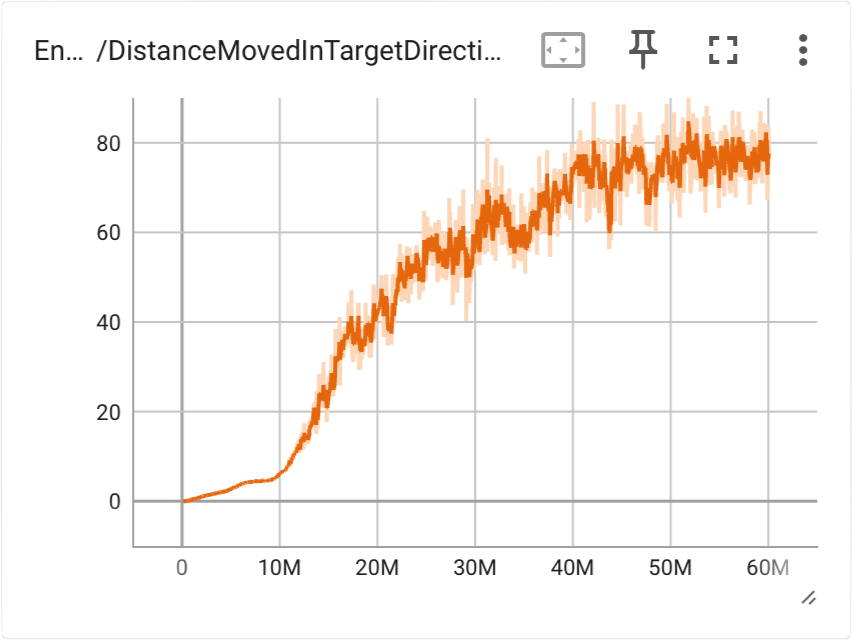
\includegraphics[width=\textwidth]{img/113_move_target_dir}
      \caption{Zurückgelegte Strecke in Zielrichtung}
      \label{fig:113_move_target_dir}
    \end{subfigure}
    \begin{subfigure}{.49\textwidth}
      \centering  
      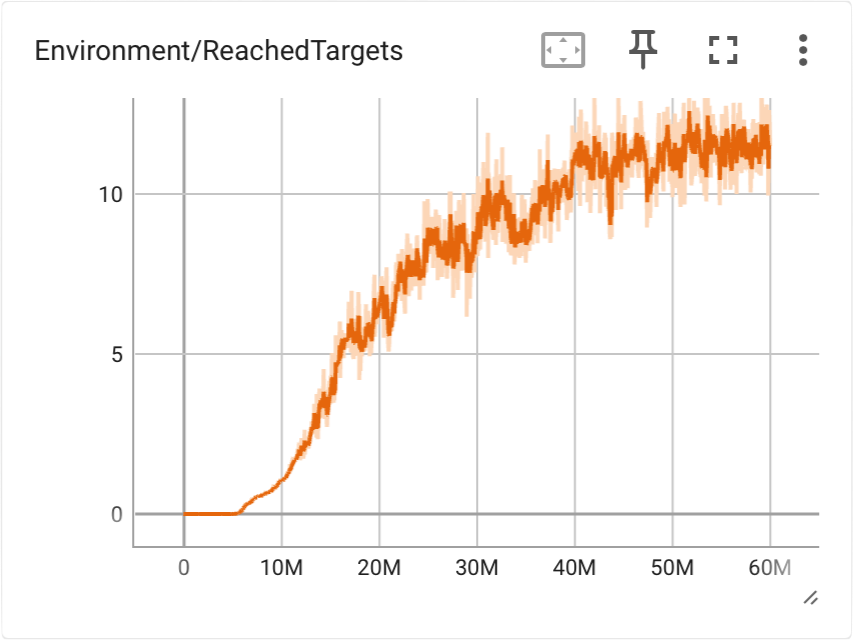
\includegraphics[width=\textwidth]{img/113_reach_target}
      \caption{Erreichte Anzahl an Zielen}
      \label{fig:113_reach_target}
    \end{subfigure}
    \begin{subfigure}{.49\textwidth}
      \centering  
      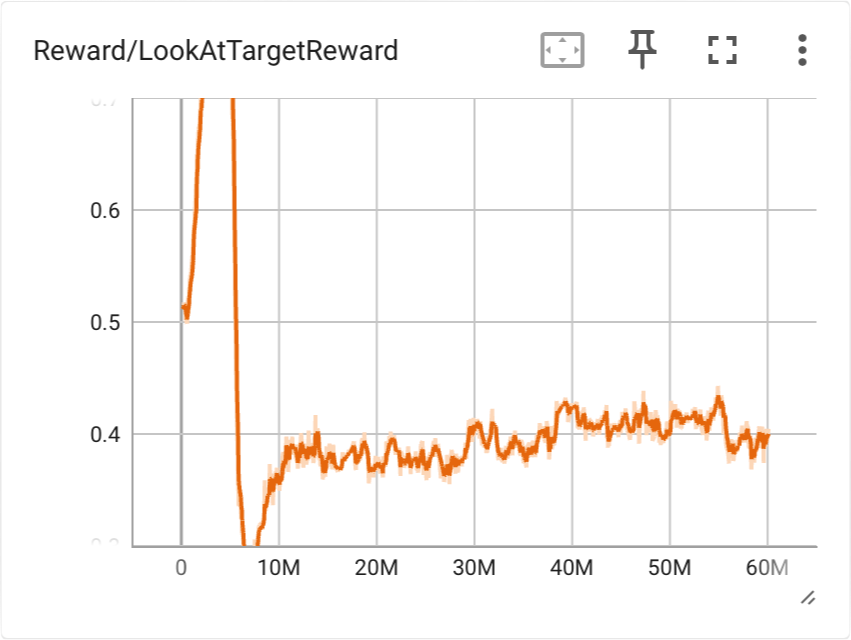
\includegraphics[width=\textwidth]{img/113_look_reward}
      \caption{Blickbelohnung}
      \label{fig:113_look_reward}
    \end{subfigure}
  \caption{Training Blickrichtungsziel mit Wechsel bei durchschnittlicher Blickbelohnung von 0.7}
  \label{fig:training_blickrichtungsziel_wechsel_07}
\end{figure}

Um von Anfang an und separat vom Erlernen des Laufens die Blickbelohnung zu erlernen, wird die Bedingung für das Erreichen eines Blickziels erneut angepasst. Im folgenden Versuch wird der Blickzielwinkel gewechselt, sobald der Läufer 3 Sekunden auf das Ziel blickt. Implementiert wurde das Ganze mit einem Spherecast, um gleichzeitig die Genauigkeit, mit der der Läufer auf das Ziel schauen muss, anpassen zu können (siehe Abbildung \ref{fig:spherecast}). Spherecast ist eine Technik, die verwendet wird, um eine kugelförmige Kollisionsabfrage durchzuführen. Zusätzlich zur Funktionsweise eines Raycast ermöglicht der Spherecast, über den Kugeldurchmesser die Blickfeldgröße anzupassen. je nach Kugelgröße und Dauer des Blickkontakts kann die Schwierigkeit variiert werden. Grundlegend lässt sich darüber aber die Abhängigkeit zum Lernverlauf der Fortbewegung lösen. Gleichermaßen kann zusätzlich auch die geforderte Präzision angepasst werden.

\begin{figure}[H]
  \centering  
  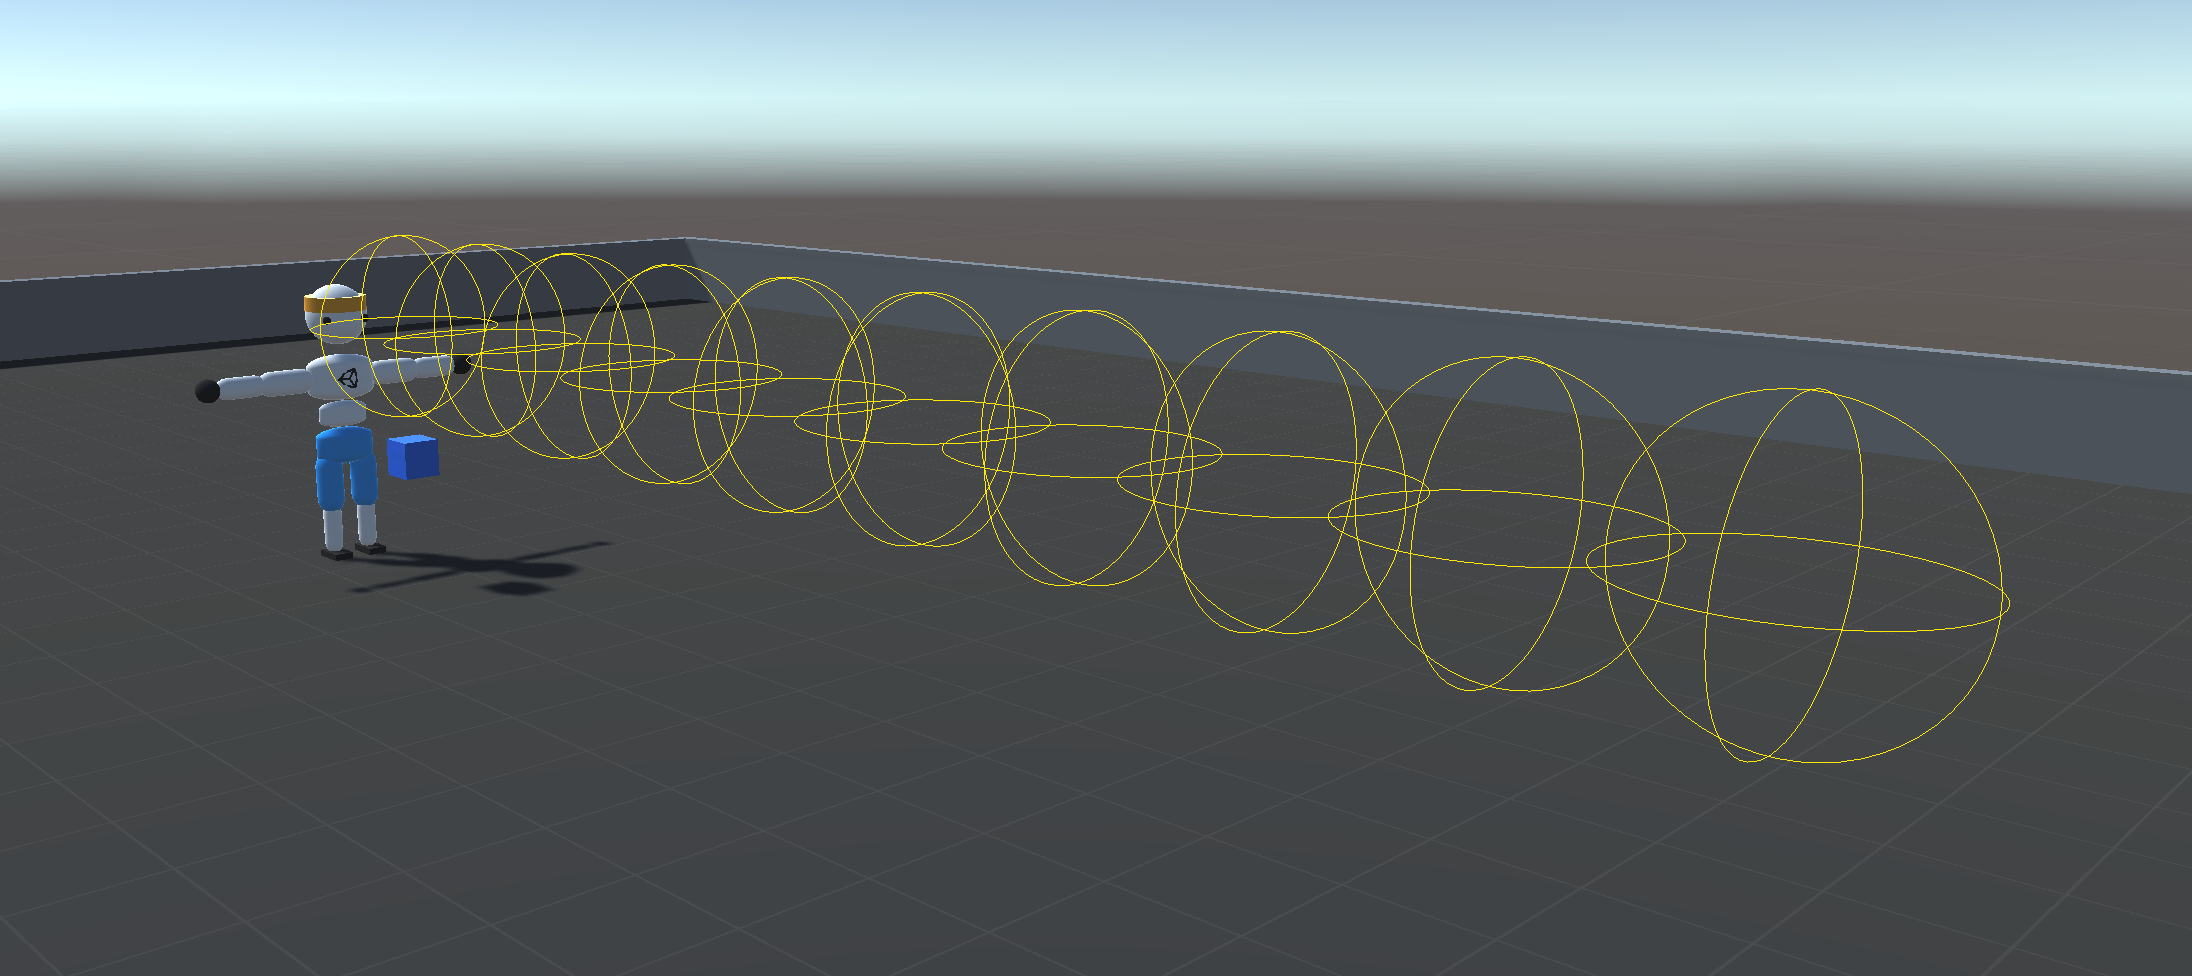
\includegraphics[width=0.8\textwidth]{img/spherecast}
  \caption{Spherecast in Blickrichtung}
  \label{fig:spherecast}
\end{figure}

Das Training wurde einmal mit 3 Sekunden und einmal mit 2 Sekunden Blickkontaktzeit zum Erreichen des Blickziels durchgeführt, wobei das Training mit 2 Sekunden Blickkontaktzeit besser abschneidet. Trotz dieser Anpassungen ist der Schwierigkeitsgrad des Trainings noch sehr hoch. Selbst das bessere der beiden Trainings ist nach 120 Millionen Trainingsschritten noch weit davon entfernt, stabil mehrere Ziele am Stück zu erreichen. Es ist zu vermuten, dass weitere Anpassungen erforderlich sind, um die gewünschte Stabilität zu erreichen. Ein weiteres Problem, welches bei der Auswertung entdeckt wurde ist, dass die Belohnung auch ohne erreichen der Blickziele optimiert werden kann. Es ist für den Agenten möglich, die Schwierigkeit des wechselnden Blickziels zu umgehen, indem er den Blickkontakt zum Ziel nie für 2 volle Sekunden hält. Dieses Problem muss in kommenden Versuchen berücksichtigt werden.\hl{ende ??}

\begin{figure}[H]
  \centering  
    \begin{subfigure}{.49\textwidth}
      \centering  
      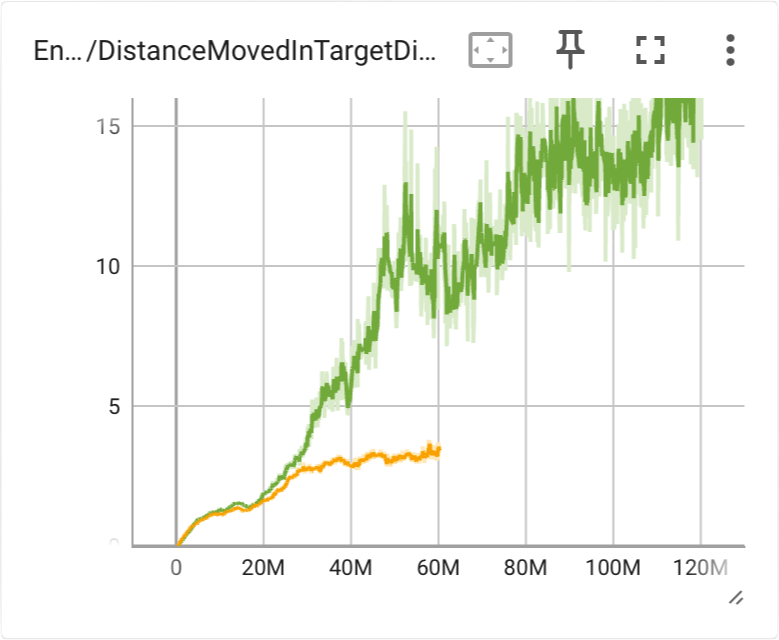
\includegraphics[width=\textwidth]{img/117_119_move_target_dir}
      \caption{Zurückgelegte Strecke in Zielrichtung}
      \label{fig:117_119_move_target_dir}
    \end{subfigure}
    \begin{subfigure}{.49\textwidth}
      \centering  
      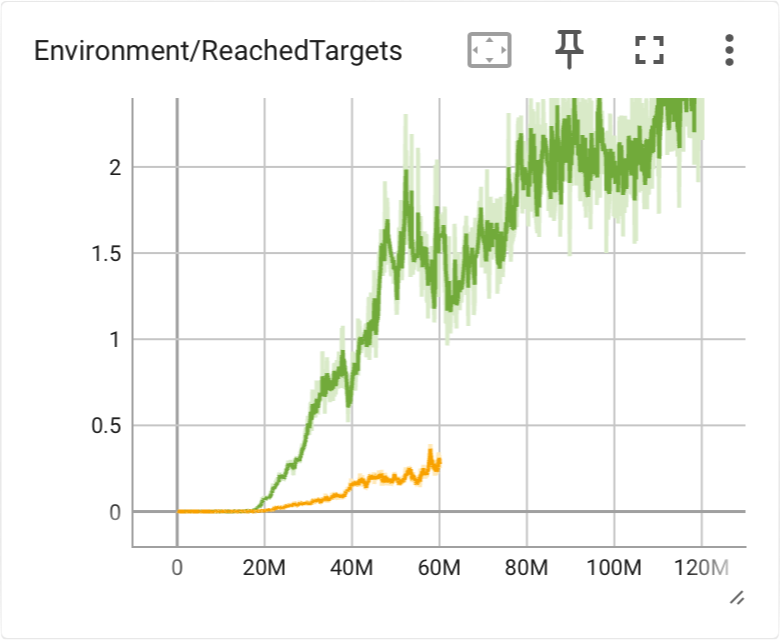
\includegraphics[width=\textwidth]{img/117_119_reach_target}
      \caption{Erreichte Anzahl an Zielen}
      \label{fig:117_119_reach_target}
    \end{subfigure}
    \begin{subfigure}{.49\textwidth}
      \centering  
      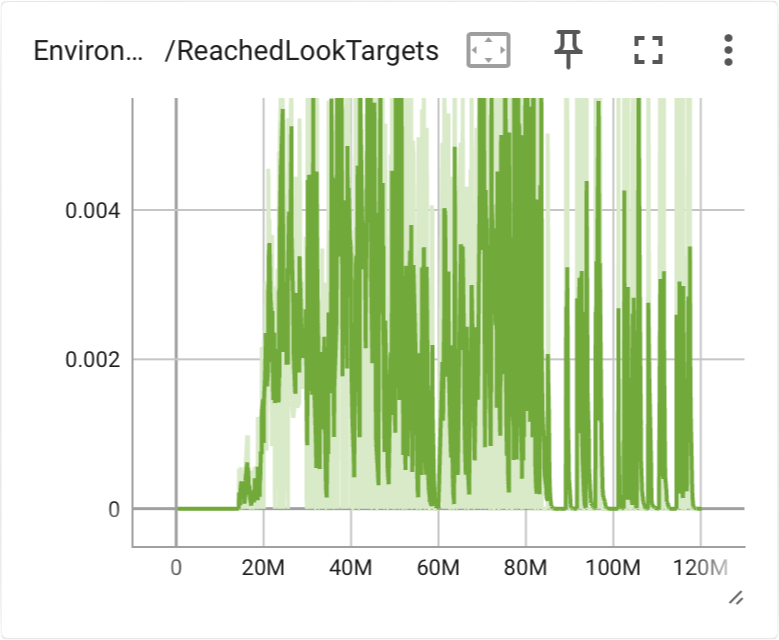
\includegraphics[width=\textwidth]{img/117_119_reach_look_target}
      \caption{Erreichte Anzahl an Blickzielen}
      \label{fig:117_119_reach_look_target}
    \end{subfigure}
    \begin{subfigure}{.49\textwidth}
      \centering  
      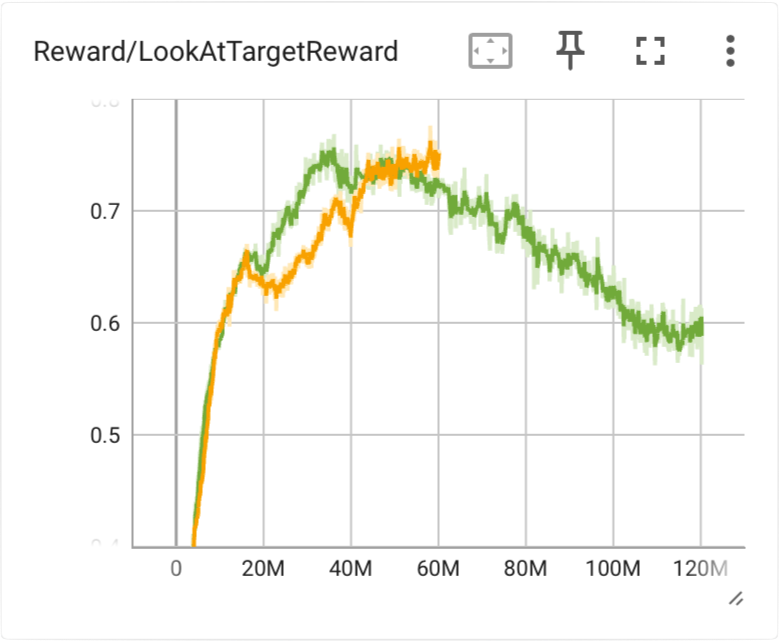
\includegraphics[width=\textwidth]{img/117_119_look_reward}
      \caption{Blickbelohnung}
      \label{fig:117_119_look_reward}
    \end{subfigure}
  \caption{Training Blickrichtungsziel mit Wechsel bei Blickkontakt von 2 bzw. 3 Sekunden (orange = 3 sek, grün = 2 sek)}
  \label{fig:training_blickrichtungsziel_wechsel_spherecast}
\end{figure}